\documentclass[border=10pt]{standalone}

\usepackage{tikz}
\usepackage{tikzsymbols}
\usetikzlibrary{calc,patterns,shapes.geometric}

\def\centerarc[#1](#2)(#3:#4:#5){\draw[#1] ($(#2)+({#5*cos(#3)},{#5*sin(#3)})$) arc (#3:#4:#5);}

\begin{document}
	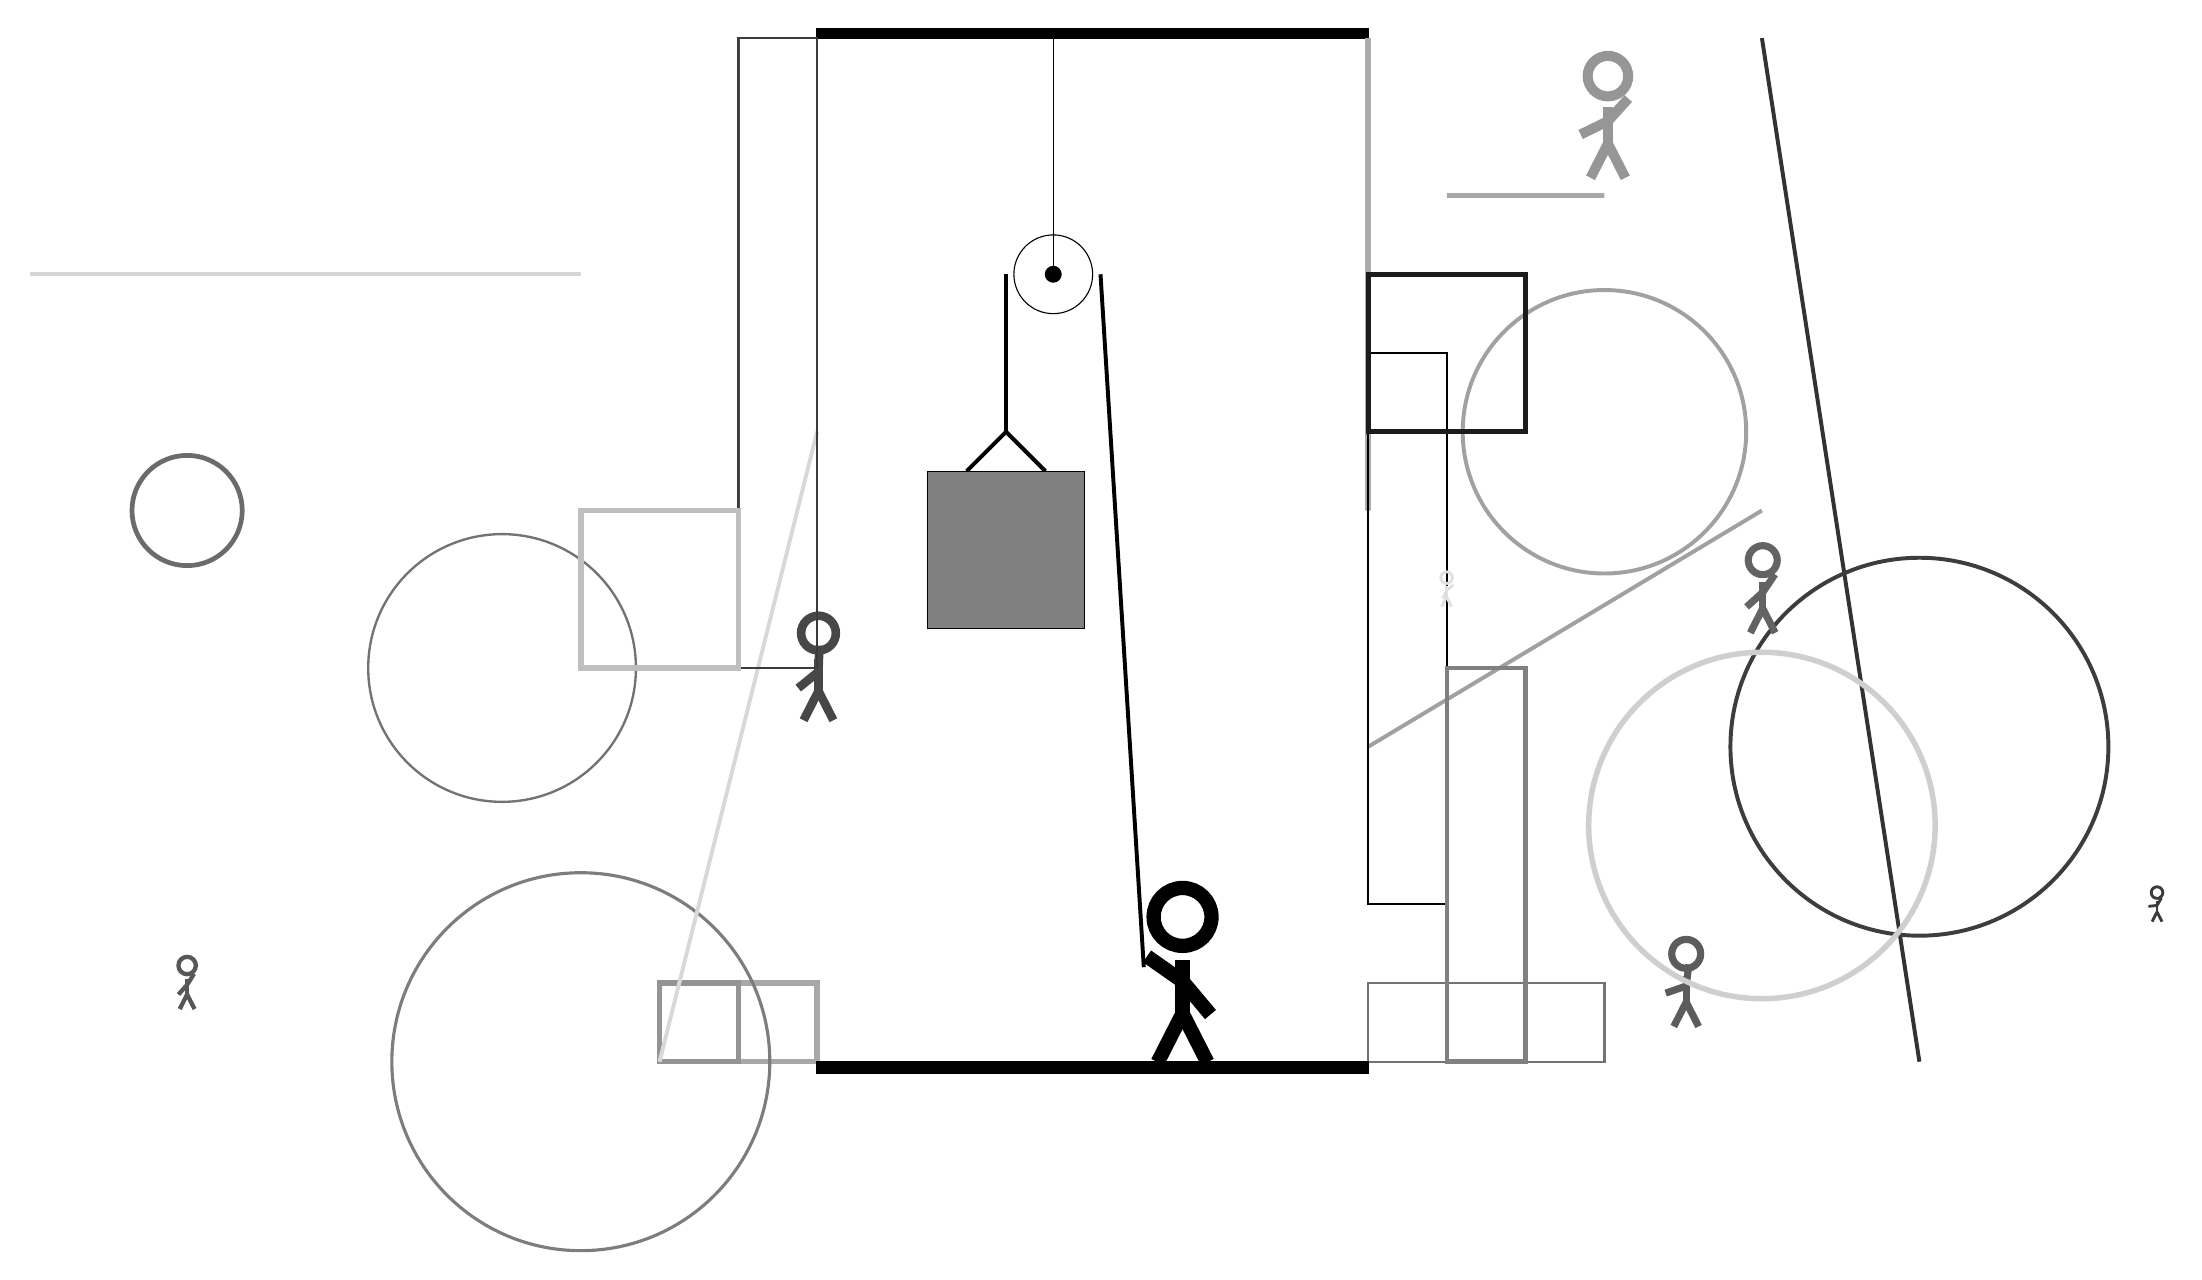
\begin{tikzpicture}
		%%%%% START %%%%%
		
		\draw[fill=black] (-2, 10) rectangle (5, 10.125);
		
		\draw[line width=0.7mm, color=black!33] (5, 4) rectangle (5, 10);
		
		\draw[line width=0.7mm, color=black!34] (-4, -3) rectangle (-2, -2);
		\draw[line width=0.5mm, color=black!16](-5, 7) -- (-12, 7);
		\node[line width=0.6mm, color=black!72] at (-2, 2) {\Strichmaxerl[6][39][88]};
		\draw [line width=0.4mm, color=black!51](-5, -3) circle (2.4);
		\draw[line width=0.5mm, color=black!37](5, 1) -- (10, 4);
		\draw[line width=0.5mm, color=black!80](10, 10) -- (12, -3);
		
		\draw[line width=0.7mm, color=black!42] (-4, -2) rectangle (-3, -3);
		\draw[line width=0.6mm, color=black!34] (6, 8) rectangle (8, 8);
		\draw [line width=0.5mm, color=black!37](8, 5) circle (1.8);
		
		\draw [line width=0.5mm, color=black!76](12, 1) circle (2.4);
		\node[line width=0.3mm, color=black!61] at (10, 3) {\Strichmaxerl[5][42][56]};
		\draw [line width=0.3mm, color=black!55](-6, 2) circle (1.7);
		
		\draw[line width=0.3mm, color=black!55] (5, -2) rectangle (8, -3);
		\node[line width=0.5mm, color=black!77] at (15, -1) {\Strichmaxerl[2][6][60]};
		\node[line width=0.4mm, color=black!41] at (8, 9) {\Strichmaxerl[7][26][48]};
		
		\draw[line width=0.4mm, color=black!70] (-3, 10) rectangle (-3, 3);
		
		\draw[line width=0.5mm, color=black!33](5, 8) -- (5, 7);
		\draw[line width=0.3mm, color=black!100] (6, 6) rectangle (5, -1);
		\draw[line width=0.5mm, color=black!15](-4, -3) -- (-2, 5);
		\draw[line width=0.3mm, color=black!77] (-2, 2) rectangle (-3, 10);
		\node[line width=0.5mm, color=black!12] at (6, 3) {\Strichmaxerl[2][64][41]};
		\draw[line width=0.6mm, color=black!50] (7, -3) rectangle (6, 2);
		\draw[line width=0.7mm, color=black!25] (-3, 2) rectangle (-5, 4);
		\node[line width=0.6mm, color=black!64] at (9, -2) {\Strichmaxerl[5][19][83]};
		
		\draw[line width=0.6mm, color=black!89] (5, 7) rectangle (7, 5);
		\node[line width=0.4mm, color=black!66] at (-10, -2) {\Strichmaxerl[3][48][58]};
		\draw [line width=0.6mm, color=black!58](-10, 4) circle (0.7);
		
		\draw [line width=0.7mm, color=black!19](10, 0) circle (2.2);
		
		\draw (1, 7) circle (0.5);
		\draw[fill=black] (1, 7) circle (0.1);
		\draw (1, 10) -- (1, 7);
		
		\draw[line width=0.5mm] (-0.1, 4.5) -- (0.4, 5.0) -- (0.9, 4.5);
		\draw[fill=black!50] (-0.6, 4.5) rectangle (1.4, 2.5);
		
		\draw[line width=0.5mm] (0.4, 7) -- (0.4, 5.0);
		\centerarc[line width=0.5mm](1, 7)(0:180:0.6);
		\draw[line width=0.5mm](1.6, 7) -- (2.15, -1.8);
		
		\node at (2.6, -1.9) {\Strichmaxerl[10][-35][-50]};
		
		\draw[fill=black] (-2, -3) rectangle (5, -3.15);
		
		%%%%% END %%%%%
	\end{tikzpicture}
\end{document}